\chapter{OpenID Connect}

Come detto in precedenza, OAuth 2.0 fornisce mezzi di autorizzazione ma non di
autenticazione, spesso vengono implementate tecniche proprietari che consentono
l'autenticazione su OAuth 2.0 tutta via può essere utile avere un protocollo standard
che possa portare a questi risultati.
Questo protocollo è \textbf{OIDC} (\textit{Open ID Connect}) che fornisce un identity service layer
per OAuth 2.0.

\begin{figure}[H]
    \centering
    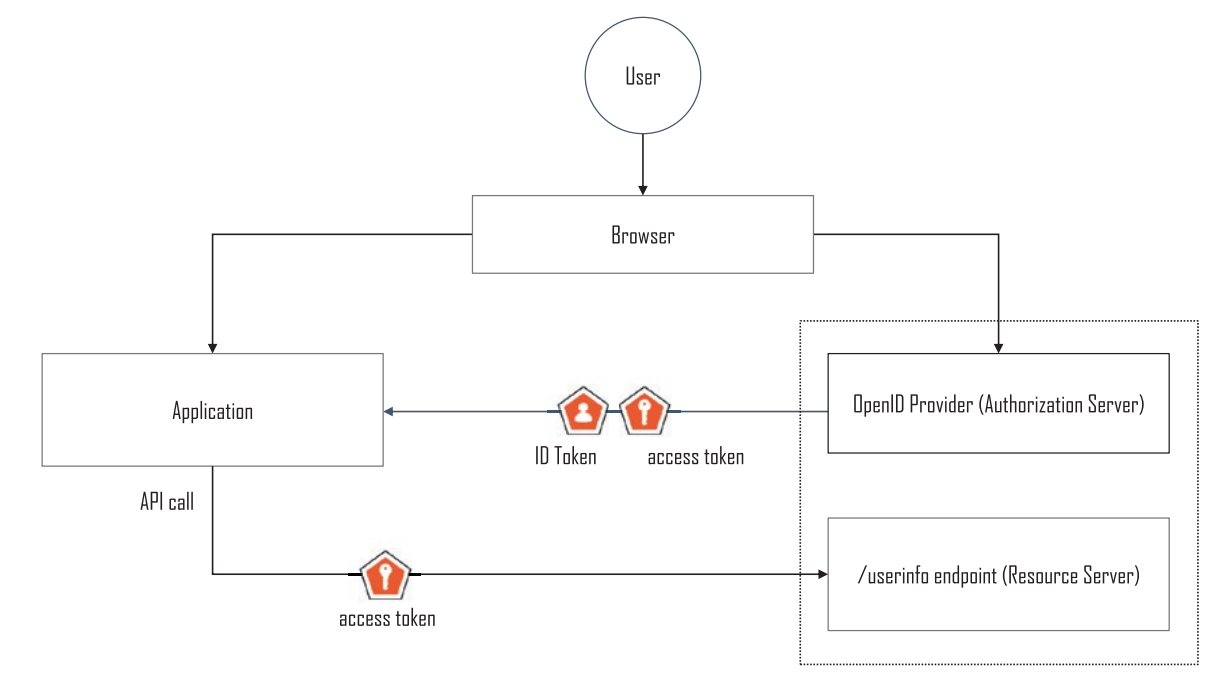
\includegraphics[width=\textwidth, keepaspectratio]{capitoli/id_managing/imgs/oidc1.png}
    \caption{Schema di autenticazione con OIDC.}
\end{figure}

Nella figura precedente possiamo vedere come funziona l'autenticazione in OIDC a
grandi linee.
Quando un utente accede all'applicazione viene reindirizzato all'authorization server
che implementa OIDC (d'ora in avanti verrà chiamato \textit{OpenID Provider}),
dopodiché l'OpenID Provider interagisce con l'utente per autenticarlo.
Dopo l'autenticazione il browser dell'utente viene reindirizzato all'applicazione.
L'applicazione ora può richiedere che le informazioni dell'utente autenticato vengano
ritornate sotto forma di un security token chiamato \textbf{ID Token} oppure può
richiedere un access token con OAuth 2.0.